% !TeX document-id = {1d88a3b2-9b5b-461b-9b0a-590d1c20474b}
% !TeX TXS-program:compile = txs:///pdflatex/[--shell-escape]
\documentclass[border={0 0mm 0 -1mm}]{standalone}
\usepackage{amsmath,amsfonts,amssymb}
\usepackage{tikz,pgfplots}
\usetikzlibrary{arrows,arrows.meta,bending,calc,decorations,shadings,shadows,shapes,shapes.arrows,shapes.geometric}
\usetikzlibrary{calc,fadings,decorations.pathreplacing}
\usepgfplotslibrary{units,fillbetween,groupplots,colorbrewer}
\usetikzlibrary{pgfplots.colorbrewer,}
\usepackage{pgfplotstable}

\pgfdeclareplotmark{*)}
{\shade[draw=red!60!black,ball color=red!70,opacity=0.5] (0,0) circle [radius=2pt];}


\newcommand*{\xMin}{-2}%
\newcommand*{\xMax}{10}%
\newcommand*{\yMin}{-5}%
\newcommand*{\yMax}{7}%

\definecolor{As}{RGB}{255,255,0}
\definecolor{Al}{RGB}{173,216,230}
\definecolor{Ga}{RGB}{0,128,150}
\begin{document}
	
	\begin{tikzpicture}
				
%						\draw[step=.5cm,gray,very thin,opacity=0.1] (0,0) grid (\xMax,\yMax);
%						 \foreach \i in {\xMin,...,\xMax} {
%								\draw [very thin,gray] (\i,\yMin) -- (\i,\yMax)  node [below] at (\i,\yMin) {$\i$};
%							}
%						\foreach \i in {\yMin,...,\yMax} {
%								\draw [very thin,gray] (\xMin,\i) -- (\xMax,\i) node [left] at (\xMin,\i) {$\i$};
%							}
		
		
\draw[densely dashed,line width=0.5mm](-2,4.5)--(-2,2);
\draw[densely dashed,line width=0.5mm](4,4.5)--(4,2);
\draw[densely dashed,line width=0.5mm](10,4.5)--(10,2);		


\node[scale=2] at (1,3.5) {AlGaAs};
\node[scale=2] at (7,3.5) {GaAs};
		
		
		\node[anchor=center,opacity=1] at (4,8) {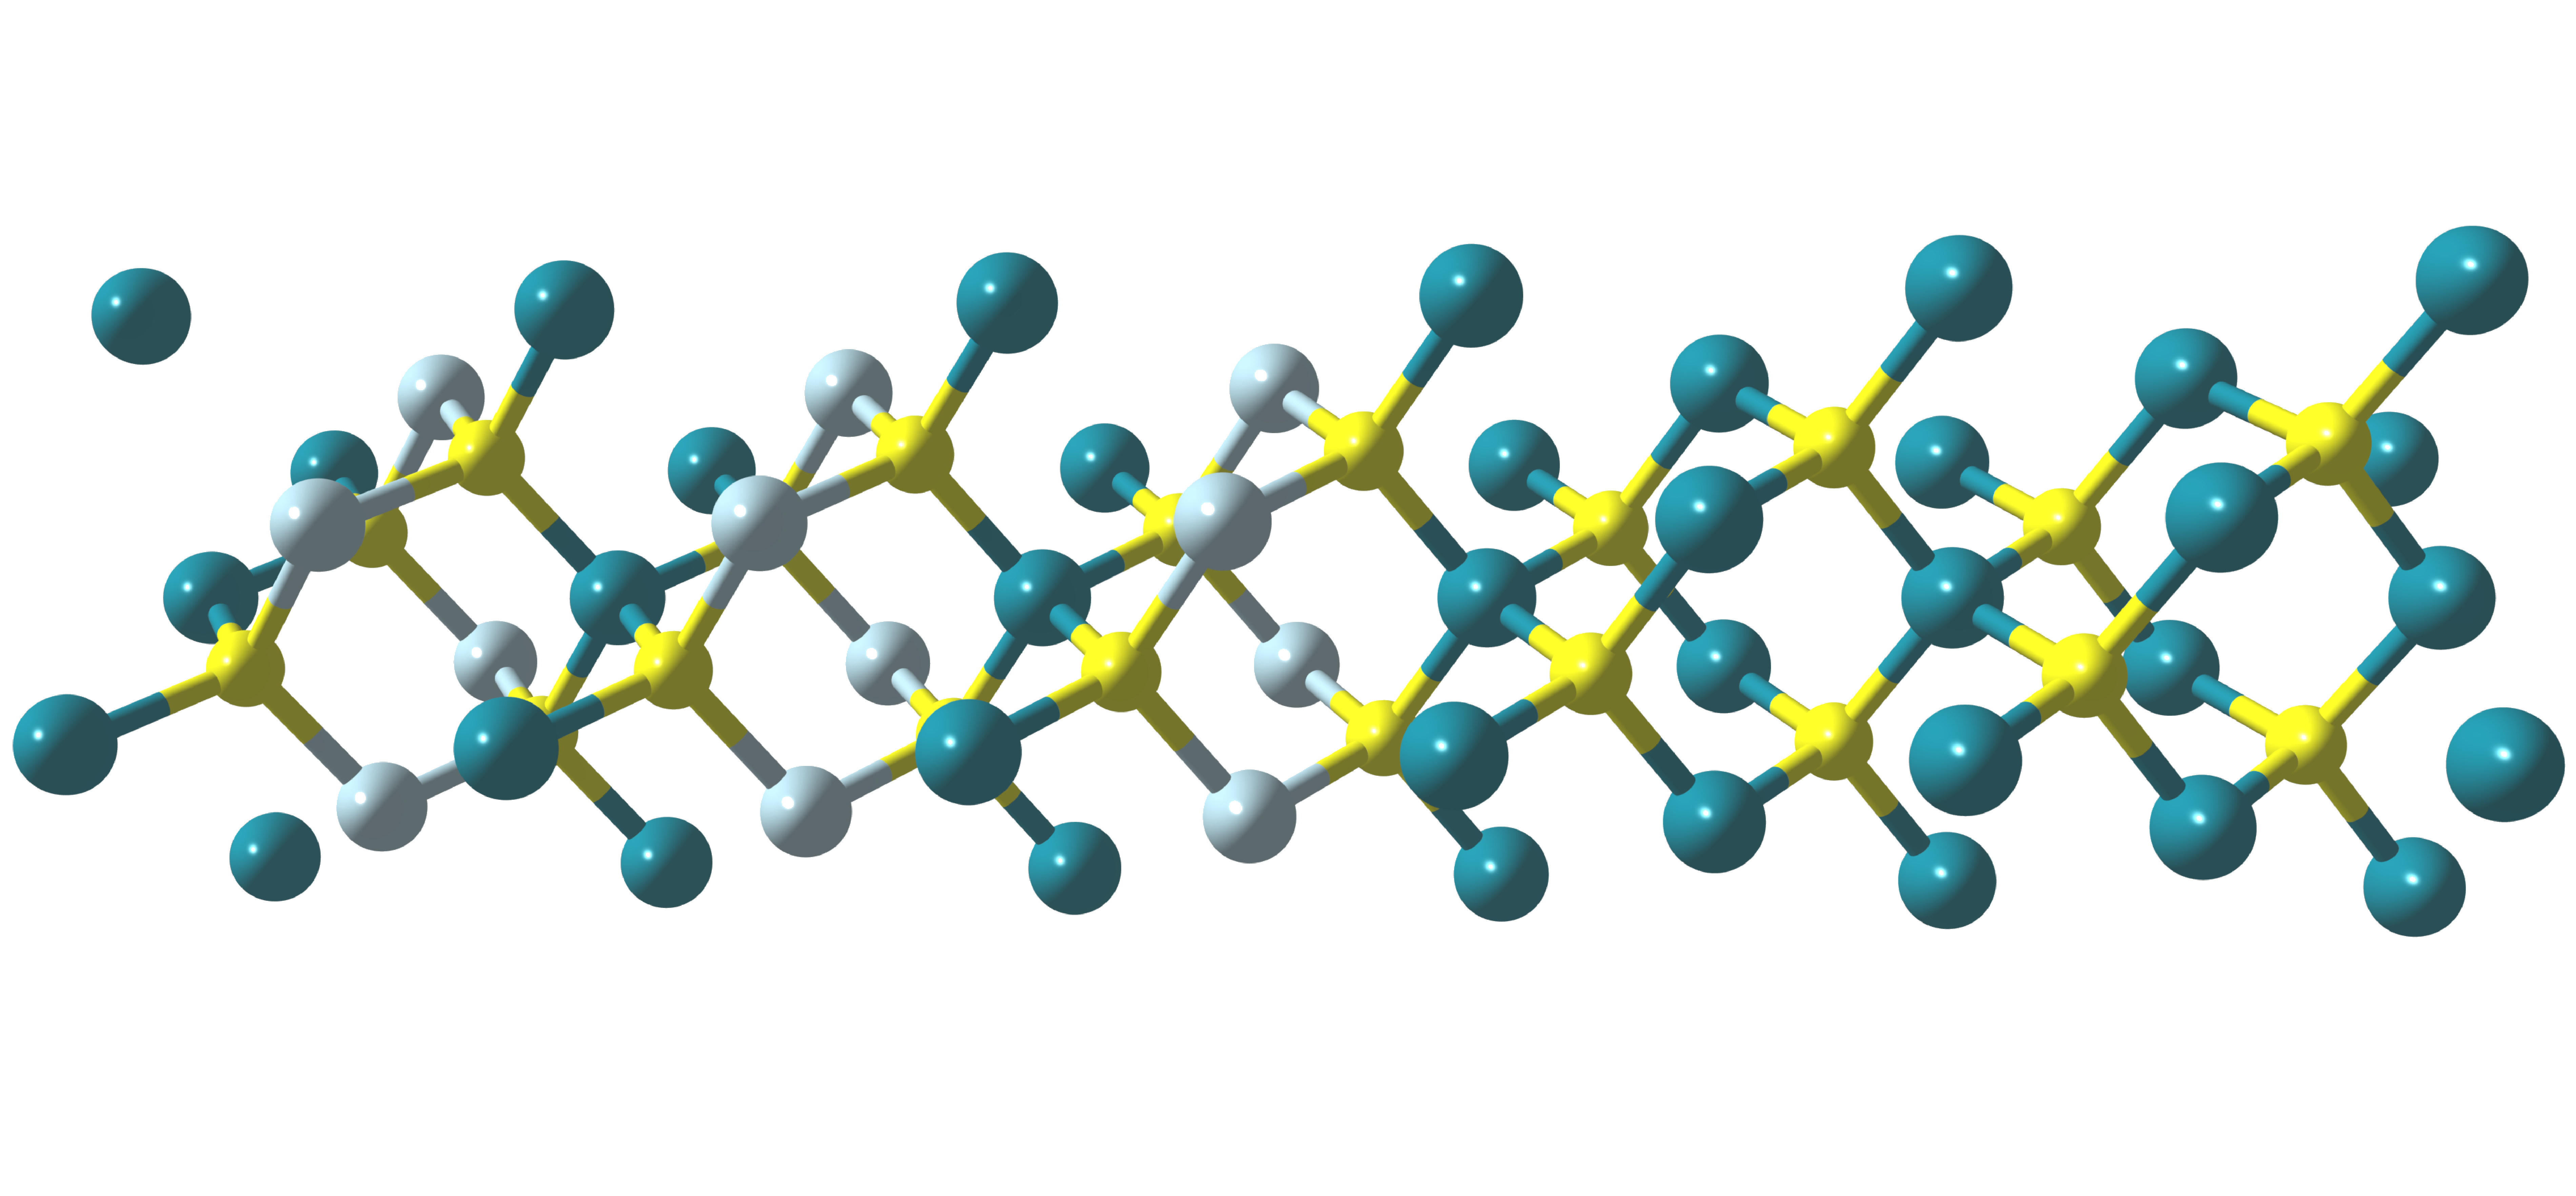
\includegraphics[width=\linewidth,trim={0 45cm 0 10cm }]{/media/labfiles/ruco/phd-ssp/phd-codes/atom-structures/heterostructure-02.pdf}};
		
		

		
%		
		\draw[line width=0.5mm] (-2,2)--(4,2)--(4,-0)--(10,-0);
				\draw[line width=0.5mm]  (-2,-5)--(4,-5)--(4,-3)--(10,-3);
		
	      \shade [ball color=As] (-3.3,7.5) circle (0.3) node[label=right:{\Large\, As}] { } ;
	       \shade [ball color=Al] (-3.3,6.5) circle (0.3) node[label=right:{\Large\, Al}] { } ;
		\shade [ball color=Ga] (-3.3,5.5) circle (0.3) node[label=right:{\Large\, Ga}] { } ;	      
		
		\node[scale=1.5] at (-1,1.5) {$\mathrm{CB}_{\mathrm{AlGaAs}}$};
		\node[scale=1.5] at (-1,-4.5) {$\mathrm{VB}_{\mathrm{AlGaAs}}$};
		
		


\path[{Stealth[scale=1.2]}-{Stealth[scale=1.2]}] (2,-5) edge[line width=0.3mm] node[ fill=white, anchor=center, pos=0.5,scale=1.5] {$\mathrm{Eg_{AlGaAs}}$} (2,2);


\node[scale=1.5] at (9,-0.5) {$\mathrm{CB}_{\mathrm{GaAs}}$};
\node[scale=1.5] at (9,-2.5) {$\mathrm{VB}_{\mathrm{GaAs}}$};


\path[{Stealth[scale=1.2]}-{Stealth[scale=1.2]}] (6,-3) edge[line width=0.3mm] node[ fill=white, anchor=center, pos=0.5,scale=1.5] {$\mathrm{Eg_{GaAs}}$} (6,0);


\draw[-{Triangle[width=3mm,length=7mm]}, line width=1mm,blue](-2.3,-1.25) -- (-2.3, 3);
\draw[-{Triangle[width=3mm,length=7mm]}, line width=1mm,red](-2.3,-2.0) -- (-2.3, -6);
\draw[-{Triangle[width=3mm,length=7mm]}, line width=1mm,](-2.0,-6) -- (10, -6);
\node[rotate=90,scale=2] at (-3,-1) {Potential $V(z)$};
\node[rotate=0,scale=2,anchor=center] at (3,-7) {Position $z$};
%		\draw(-4,-1)--(1,-1)--(1,-5)--(3,-5)--(3,-1)--(9,-1);
%		
%		\shade[gray!80,opacity=0.1,draw](-4,-1)--(2,3)--(4,3)--(1,-1)--cycle;
%		
%		\shade[gray!80,opacity=0.1,draw](3,-1)--(9,-1);
%		
%	\shade[gray!90!white,opacity=0.1](1,-5)--(3,-2)--(3,-1)--(4,0.3)--(4,3)--(1,-1)--cycle;
%	
%	
%		\draw(-4,-10)--(1,-10)--(1,-7)--(3,-7)--(3,-10)--(9,-10);
%		
%		\shade[gray!90!white,opacity=0.1](1,-10)--(3,-7.3)--(3,-7)--(1,-7)--cycle;
%		
	\end{tikzpicture}


	
	
\end{document}